\documentclass[10pt,a4paper]{article}
\usepackage{fontspec}
\usepackage{amsmath,bm}
\usepackage{amsfonts}
\usepackage{amssymb}
\usepackage{graphicx}
\usepackage{subcaption}
\usepackage{hyperref}
\usepackage{cleveref}
\usepackage{lmodern}
\usepackage{placeins}
\usepackage[left=1.00in, right=1.00in, top=1.00in, bottom=1.00in]{geometry}
\title{Assignment 2}
\author{Daniel Celis Garza}
\date{\today}
\begin{document}
	\section{Part a}
	\subsection{Definition}
	Aside from the charge exchange rate and degree of ionisation an ionised gas is called a plasma if it meets the following two conditions:
	\begin{itemize}
		\item Must be able to shield against an applied electric field, either AC or DC. Defined in terms of the Debye length $\lambda_{D}$ and plasma frequency. The electrons---since they move faster---carry out the job of screening the plasma from external potentials. However, the overall plasma must remain quasi-neutral. The shielding electrons come from the plasma bulk, so in order to maintain quasi-neutrality the number density of electrons and ions in the plasma bulk must be approximately equal $n_{i} \simeq n_{e}$. Since an ideal plasma has overall charge of zero, this means that the total number of electrons per unit volume in the bulk must not be perturbed too much by the electrons that have travelled to the screening region. Therefore, the volume of the screening region (Debye sheath) must be much smaller than the bulk volume of the plasma. In terms of the characteristic length scales this means $\lambda_{D} \lll L$.
		\item Must behave like a fluid, described by magneto-hydrodynamics (MHD). Defined in terms of the plasma parameter $\Lambda_{D}$. This means that each volume element must be sufficiently small for accurate treatment under MHD, yet contain enough particles for the description to be statistically sound. Also, if we want to treat the Debye sphere within the same framework, the fluid element must be much smaller than the Debye length, or approximately equal at the worst $l \lesssim \lambda_{D}$. This means that if we calculate the plasma parameter, or number of particles per fluid element $\Lambda_{D} = \dfrac{4 \pi}{3} n_{e} \lambda_{De}^{3} = \dfrac{4 \pi}{3} \dfrac{\epsilon^{3/2}}{e^{3}} \dfrac{T_e^{3/2}}{n_{e}^{1/2}} \gg 1$. This could also mean that the long-range collective behaviour must dominate over short range Coulomb interactions. By noting that the average distance between particles is approximately equal to the cube root of the density $b_{a} \sim n_{e}^{-1/3}$ and the Coulomb interaction becomes important when $\dfrac{1}{2} m_{e} v^{2} = \dfrac{e^{2}}{4\pi \epsilon_{0} b_{c}}$ where $b_{c}$ is the Coulomb interaction distance, then by forcing the long range interaction to dominate $b_{a} \gg b_{c}$ and noting that for a plasma at temperature $T_{e}$, $m_{e} v^{2} \sim k_{B}Te$ we obtain $n_{e}^{-1/3} = \dfrac{e^{2}}{2\pi \epsilon_{0} k_{B} T}$. Which we can then plug into the formula for $\Lambda_{D} \gg \dfrac{4\pi}{3 \times (2\pi)^{3/2}} \sim 0.27$.
	\end{itemize}
	\subsection{Positive Charge Q Placed in a Quasineutral Plasma}\label{ss:1}
	First, the plasma will move to screen the potential generated by the charge by forming a ``cloud'' of electrons around it. This has the effect of shielding---or screening---the potential generated by the positive charge. The phenomenon is called Debye screening, while the electron cloud that does the shielding is called the Debye sphere. At finite temperature the thermal energy of the particles is,
	\begin{align}
		\dfrac{1}{2} k_{B} T = \dfrac{1}{2} m v_{th}^{2}~.
	\end{align}
	If the kinetic energy is comparable to the potential energy we have,
	\begin{subequations}
		\begin{align}
		k_{B}T &\sim Ze\phi \\
		\phi &\sim \dfrac{k_{B}T}{Ze}\label{e:phi0}
		\end{align}
	\end{subequations}
	therefore, the bulk potential is dependent on $T$ and charge. The Debye length can be derived from the Poisson equation, and using the Boltzman relation for the electron number density where $n_{\infty}$ is the number density in the absence of $\phi$ and if we take ions to be stationary with respect to electrons $n_{\infty} = n_{i}$,
	\begin{subequations}
		\begin{align}
			\nabla^{2} \phi &= - \dfrac{e}{\epsilon_{0}} (n_{i} - n_{e})\\
			n_{e} &= n_{\infty} \exp\left(\dfrac{e\phi}{k_{B}T}\right) \\
			\nabla^{2} \phi &= - \dfrac{e n_{\infty}}{\epsilon_{0}} \left(\exp\left[\dfrac{e\phi}{k_{B}T}\right] - 1 \right)~.\label{e:pois}
		\end{align}
	\end{subequations}
	Since there is no analytical solution to \cref{e:pois} we can Taylor expand around $\phi = 0$ and come up with $\exp\left(\dfrac{e\phi}{k_{B}T}\right) \approx 1 + \dfrac{e \phi}{k_{B}T} + \ldots$ to the $O(2)$ error term and come up with the 1D equation for the Debye shielding potential,
	\begin{align}
		\dfrac{\mathrm{d}^{2} \phi}{\mathrm{d} x^{2}} &\approx \dfrac{e^{2} n_{\infty} \phi}{\epsilon_{0} k_{B} T} \\
		\lambda_{D}^{2} &= \dfrac{\epsilon_{0} k_{B} T}{e^{2} n_{\infty} \phi} \\
		\phi(x) &\approx \phi_{0} \exp\left(-\dfrac{|x|}{\lambda_{D}}\right)~.
	\end{align}
	If we then approximate the screened potential just beyond the Debye sphere we must recall \cref{e:phi0} and by setting $|x| = \lambda_{D}$ (Debye length, i.e. characteristic length) we obtain,
	\begin{subequations}
		\begin{align}
			\phi(\lambda_{D}) \approx \dfrac{k_{B} T}{Z e \exp(1)}~.
		\end{align}
	\end{subequations}
	
	\section{Part b}
	Following the force-balance equation and assuming steady state (no fluid flow and constant temperature) we can eliminate any term with $\bm{u}$,
	\begin{subequations}
		\begin{align}
			\bm{u} &= 0\\
			E &= -\nabla \phi \\
			&\therefore \nonumber\\
			\nabla p &= n Z e E = -n Z e \nabla \phi \\
			&\textrm{from the ideal gas law where $n$ is number density} \nonumber\\
			p &= n k_{B} T \\
			\nabla n k_{B} T &= -n Z e \nabla \phi \\
			\ln\left(\dfrac{n}{n_{0}}\right) &= - \dfrac{Ze \phi}{T k_{B}}\\
			k_{B} &\equiv 1 \nonumber\\
			n(x) &= n_{0} \exp\left(-\dfrac{Z e \phi}{T}\right) \label{e:ndens}
		\end{align}
	\end{subequations}
	
	A pair of electrons at $2L$ apart, one at potential $+\phi_{0}$ and the other at $-\phi_{0}$, assuming $\dfrac{e \phi_{0}}{T} \ll 1$, we can determine the potential $\phi(x)$ in the following way. First we take $x=0$ to be the point between both electrodes and by making use of \cref{e:ndens}. We can then set up the Poisson equation by following a similar but more general procedure as we did in \cref{ss:1},
	\begin{subequations}
		\begin{align}
			\dfrac{\mathrm{d}^{2} \phi}{\mathrm{d} x^{2}} &= -\dfrac{1}{\epsilon_{0}} \left(Z e n_{i} -e n_{e}\right)\\
			\dfrac{\mathrm{d}^{2} \phi}{\mathrm{d} x^{2}} &= \dfrac{e}{\epsilon_{0}} \left[n_{0,e} \exp\left(\dfrac{e \phi}{T}\right) - Z n_{0,i} \exp\left(-\dfrac{Z e \phi}{T}\right)\right]\\
			n_{0,e} &= Z n_{0,i} \textrm{ (plasma neutrality)} \\
			\dfrac{\mathrm{d}^{2} \phi}{\mathrm{d} x^{2}} &= \dfrac{Z e n_{0,i}}{\epsilon_{0}} \left[\exp\left(\dfrac{e \phi}{T}\right) - \exp\left(-\dfrac{Z e \phi}{T}\right)\right] \\
			&\textrm{Taylor expand to $O(2)$ term} \nonumber \\
			\dfrac{\mathrm{d}^{2} \phi}{\mathrm{d} x^{2}} &\approx \dfrac{Z e n_{0,i}}{\epsilon_{0}} \left(\dfrac{e \phi}{T} + \dfrac{Z e \phi}{T}\right) \\
			&\textrm{this is an eigenvalue equation} \nonumber \\
			\dfrac{\mathrm{d}^{2} \phi}{\mathrm{d} x^{2}} &\approx \dfrac{Z e^{2} n_{0,i}}{\epsilon_{0} T} (1 + Z) \phi \\
			&\textrm{defining $\lambda^{2}$} \nonumber\\
			\lambda^{2} &\equiv \dfrac{Z e^{2} n_{0,i}}{\epsilon_{0} T} (1 + Z) \nonumber\\
			\dfrac{\mathrm{d}^{2} \phi}{\mathrm{d} x^{2}} &\approx \lambda^{2} \phi \\
			&\textrm{the general solution to this is a superposition of exponentials}\nonumber\\
			\phi(x) &\approx \phi_{+} e^{\lambda x} + \phi_{-} e^{-\lambda x} \\
			&\textrm{plugging in the boundary conditions} \nonumber\\
			\phi(-L) &= -\phi_{0}, \qquad \phi(L) = \phi_{0} \\
			\phi_{0} &= \phi_{+} e^{\lambda L} + \phi_{-} e^{-\lambda L} \\
			-\phi_{0} &= \phi_{+} e^{-\lambda L} + \phi_{-} e^{\lambda L} \\
			&\textrm{adding both boundary equations we find} \nonumber\\
			0 &= \phi_{+} \left(e^{\lambda L} + e^{-\lambda L} \right) + \phi_{-} \left(e^{\lambda L} + e^{-\lambda L} \right)\\
			&\therefore \nonumber\\
			\phi_{+} &= -\phi_{-}\\
			\phi_{0} &= \phi_{+} \left(e^{\lambda L} - e^{-\lambda L} \right)\\
			\dfrac{\phi_{0}}{\left(e^{\lambda L} - e^{-\lambda L} \right)} &= \phi_{+}\\
			&\textrm{plugging back into the general solution}\nonumber\\
			\phi(x) &\approx \dfrac{\phi_{0}}{\left(e^{\lambda L} - e^{-\lambda L} \right)} \left(e^{\lambda x} - e^{-\lambda x}\right)~.
		\end{align}
	\end{subequations}
	The potential is sketched out in \cref{f:potential}.
	\begin{figure}
		\centering
		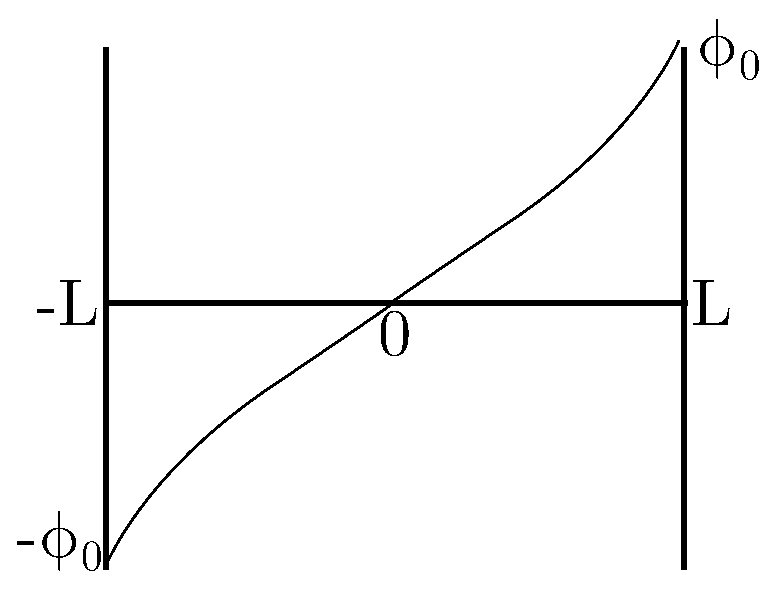
\includegraphics[width=0.5\textwidth]{potential.eps}
		\caption{Sketch of the solution to the potential.}
		\label{f:potential}
	\end{figure}
	
	\section{Part c}
	The walls of the tokamak act as a sink of charged particles, therefore particles tend to stick to it and recombine to neutralise. Electrons have higher mobility than ions, so they will get to the walls quicker. This builds an electrostatic potential on the wall of the plasma. As the wall potential grows, electrons start be decelerated while ions accelerate towards the wall. At equilibrium, the ion and electron fluxes must be zero. \Cref{e:sheath} show the considerations utilised,
	\begin{subequations}
		\begin{align}
		&\textrm{conservation of energy}\nonumber\\
		\dfrac{1}{2} m_i v_i^2 &= \dfrac{1}{2} m_i v_0^2 - e \phi\\
		&\textrm{ion flux must be conserved within the sheath}\nonumber\\
		n_iv_i &= n_0 v_0 \\
		n_i &= n_0 \left(1 - \dfrac{2e\phi}{m_i v_0^2}\right)^{-1/2}\\
		n_e &= n_0 \exp\left(\dfrac{e\phi}{T}\right) \\
		&\textrm{Taylor expanding the square root and plugging into the poisson equation}\nonumber\\
		\dfrac{1}{2} \dfrac{\mathrm{d}^2 \phi}{\mathrm{d}x^2} &= \dfrac{n_0}{\epsilon_0} \left(T_e \left(\exp\left[\dfrac{e\phi}{T_e}\right] - 1\right) + 2E \left[\left(1-\dfrac{e\phi}{E}\right)^{1/2} - 1\right]\right)~.
		\end{align}\label{e:sheath}
	\end{subequations}
	If we want a physical solution then RHS $> 0$, expanding in the limit $\epsilon \phi \ll T_e$ we find the Bohm criterion,
	\begin{subequations}
		\begin{align}
			v_0 \geq v_B &= \left(\dfrac{T_e}{m_i}\right)^{1/2} \\
			&\textrm{more generally with $T_i > 0$}\nonumber\\
			v_0 \geq c_s &=\left(\dfrac{T_i + T_e}{m_i}\right)^{1/2}~.
		\end{align}
	\end{subequations}
	The Bohm criterion indicates the existence of the pre-sheath, which lies beyond the Debye shielding. Ions must enter the pre-sheath with sufficient velocity, where they will be further accelerated by the potential and into the Debye sheath. Still, within the presheath, quasineutrality is maintained.
	
	The scrape-off layer is given by \cref{e:soff}. For an ITER-like plasma $D_\perp \sim 1 m^2s^{-1},~ T_{edge} = 100 eV,~ q \approx 4,~ R = 6.2 m$, plugging into \cref{e:soff} we get \cref{e:iter}
	\begin{subequations}
		\begin{align}
		\lambda_{SOL} &= \sqrt{\dfrac{D_\perp \pi R q}{c_s}} \label{e:soff}\\
		c_s &= \sqrt{\dfrac{e T_e}{m_i}} \nonumber\\
		\lambda_{SOL} &\approx \sqrt{\dfrac{8 m_i^{1/2}}{e^{1/2}}} \approx \sqrt{8} \dfrac{2 \times 10^{-7}}{2 \times 10^{-5}}m \approx 3 cm\label{e:iter}~.
		\end{align}
	\end{subequations}
	
\end{document}